\chapter{Implementierung}
Die Implementierung wurde entlang des Entwurfs durchgeführt. Es werden UML- und
Sequenz-Diagramme verwendet, um die Zusammenhänge zu visualisieren.

\section{Überblick}
Im Rahmen der Arbeit sind eine Reihe von Bundles entstanden, die die verschiedenen Funktionalitäten umsetzen. Es lassen sich drei Arten von Bundles unterscheiden:
\begin{enumerate}
\item Die Bundles \textit{tka.binding.core} und \textit{tka.automation.extension} bieten eine Reihe generischer Schnittstellen, die von den Bindings genutzt werden.
\item Bindings sind Bundles, die jeweils einen konkreten Webservice in das System integrieren. Es sind vier solche Bundles entstanden.
\item Das \textit{tka.flashui} Bundle stellt die Benutzeroberfläche bereit, über neue Webservice-Things zum System hinzugefügt und durch Regeln automatisiert werden können.
\end{enumerate}


\section{Schnittstellen-Bundles}
Das Ziel der Arbeit ist es einen Demonstrator zu erstellen, der in der Lage ist, die neuen Funktionalitäten zu veranschaulichen. In diesem Rahmen wurde entschieden, sich bei der Implementierung auf eine Instanz eines Things zu begrenzen...



\subsection{tka.binding.core}
Das Bundle \textit{tka.binding.core} enthält die zentrale Schnittstelle für den Prozess der Authentifizierung. Sie ist generisch aufgebaut und entspricht den Anforderungen des OAuth Standards (siehe Sektion \ref{subsubsec:oauth}). In Abbildung \ref{fig:connectionservice} ist die Struktur visualisiert.

\begin{figure}[h]
	\centering
	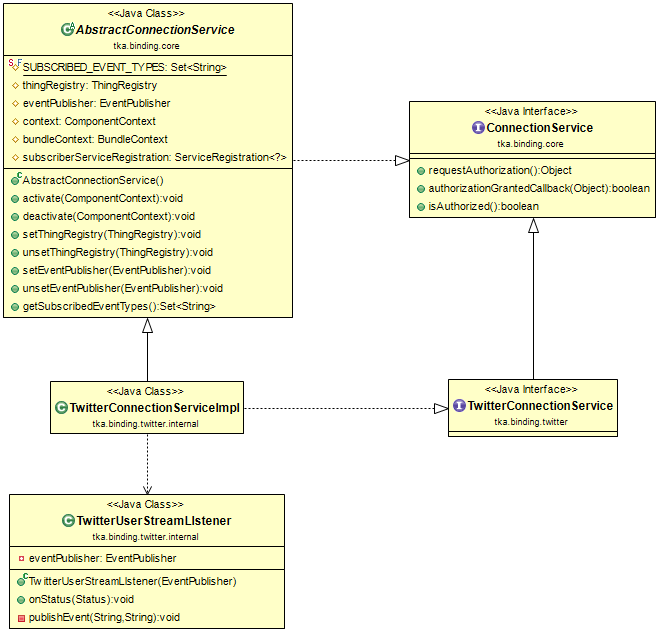
\includegraphics[width=\textwidth]{bilder/ConnectionService}
	\caption{Die Struktur einer Verbindung mit Besipielimplementierung für Twitter}
	\label{fig:connectionservice}
\end{figure}

\subsubsection{ConnectionService}
Die ConnectionService Schnittstelle bietet drei wesentliche Methoden, die bei der Authentifizierung relevant sind. Per \textit{requestAuthorization} teilt der Nutzer mit, dass er wünscht, die Anwendung mit einem seiner Webservice-Accounts (beispielsweise Twitter) zu verknüpfen. Daraufhin bekommt er in der Regel eine URL geliefert, über die er dies umsetzen kann. Die PIN, die er auf diese Weise erhält, teilt er über den \textit{authorizationGrantedCallback} der Anwendung mit. Schließlich lässt sich über \textit{isAuthorized} stets abfragen, ob die Anwendung bereits über die benötigten Zugriffsrechte verfügt. Im Rahmen dieser Arbeit wurde entschieden, sich auf die tatsächliche Unterstützung nur eines Accounts einer Art zu beschränken, obwohl die generische Struktur geeignet ist, um beliebige Mengen von Accounts zu verwalten.

\subsubsection{AbstractConnectionService}
Der AbstractConnectionService bietet eine Reihe von unterstützenden Funktionalitäten, die in der Regel von den Bindings benötigt werden. Hierzu gehört unter anderem die Beziehung des \textit{ThingRegistry}- und \textit{EventPublisher}-Services aus dem System, sowie die eigene Registrierung als \textit{EventSubscriber}. Die ThingRegistry wird benötigt um entsprechende Things im System zu registrieren, nachdem die Autorisierung erfolgreich abgeschlossen ist. Über den EventPublisher publizieren die konkreten Listener die Zustandsänderungsevents (mehr dazu in Sektion \ref{sec:bindings_impl}).\\



Jedes Binding enthält eigene Implementierungen der oben genannten Schnittstellen, die die Besonderheiten des konkreten Webdienstes berücksichtigen.


\subsection{tka.automation.extension}



\section{Bindings}
\label{sec:bindings_impl}


\subsection{tka.binding.twitter}
Hier werden die Detatils des Bindings erläutert
\subsubsection{Triggers und Events}
\subsubsection{Actions}

\subsection{tka.binding.dropbox}
\subsubsection{Triggers und Events}
\subsubsection{Actions}

\subsection{tka.binding.weather}
\subsubsection{Triggers und Events}
\subsubsection{Actions}

\subsection{tka.binding.gmail}
\subsubsection{Triggers und Events}
\subsubsection{Actions}

\subsection{tka.flashui}
Aufbau der implementierten GUI, sowie ihre Funktionalität.

\section{Fazit}